\documentclass[12pt]{article}

\usepackage[utf8]{inputenc}
\usepackage{latexsym,amsfonts,amssymb,amsthm,amsmath}
\usepackage{tikz}
\usepackage{stanli}
\usetikzlibrary{shapes,calc,through,3d}
\usetikzlibrary{decorations.pathreplacing}
\usepackage{multicol}
\usepackage{geometry} 
\usepackage{mathtools}
\usepackage{subcaption}


\setlength{\parindent}{0in}
\setlength{\oddsidemargin}{-0.25in}
\setlength{\textwidth}{7in}
\setlength{\textheight}{9.3in}
\setlength{\topmargin}{-1in}
\setlength{\headheight}{18pt}

\newcommand\blfootnote[1]{%
  \begingroup
  \renewcommand\thefootnote{}\footnote{#1}%
  \addtocounter{footnote}{-1}%
  \endgroup
}

\definecolor{darkred}{rgb}{0.6,0,0}

\newcommand{\bolddelta}{\boldsymbol\delta}


\title{}
\author{Stefano Burzio}
\date{}

\begin{document}
%%%Gauss-Legendre 1D
\hrulefill
\vspace{0.3cm}

\hspace*{\fill}\textbf{\Large Gauss-Legendre points and weights in 1D}\hspace*{\fill}

\hrulefill
\vfill
\begin{center}
  \textbf{Order 1}
\end{center}
\noindent \newline
\begin{minipage}{0.48\textwidth}
  \begin{tikzpicture}[scale=1.3]
    % Define points
    \coordinate (A) at (-2, 0);
    \coordinate (B) at (2, 0);
    % Label the element
    \draw[ultra thick] (A) --(B);
    % Xi axis 
    \draw[-latex,ultra thin] (-3,0) --(3,0) node[right]{$\xi$};
    % Y axis 
    \draw[-latex, ultra thin] (0,-0.5) -- (0,1);
    % Gauss points 
    \draw[fill=white, thick, draw=darkred]  (0,0) circle (3pt);
    % Mark points
    \draw[fill=white, thick]  (A) circle (2pt);
    \draw[fill=white, thick]  (B) circle (2pt);
  \end{tikzpicture}\end{minipage}
\hfill
\begin{minipage}{0.48\textwidth}
  \vfill\centering
  \begin{tabular}{c|c}
    Gauss points & Weights \\[5pt]
    $0$          & $2$     \\
  \end{tabular}
  \vfill
\end{minipage}
\vfill
\begin{center}
  \textbf{Order 3}
\end{center}
\noindent \newline
\begin{minipage}{0.48\textwidth}
  \begin{tikzpicture}[scale=1.3]
    % Define points
    \coordinate (A) at (-2, 0);
    \coordinate (B) at (2, 0);
    % Label the element
    \draw[ultra thick] (A) --(B);
    \draw[-latex,ultra thin] (-3,0) --(3,0) node[right]{$\xi$};
    % Y axis 
    \draw[-latex, ultra thin] (0,-0.5) -- (0,1);
    % Gauss points 
    \draw[fill=white, thick, draw=darkred]  (0.577,0) circle (3pt);
    \draw[fill=white, thick, draw=darkred]  (-0.577,0) circle (3pt);
    % Mark points
    \draw[fill=white, thick]  (A) circle (2pt);
    \draw[fill=white, thick] (B) circle (2pt);
    \draw[fill=white, thick]  (0,0) circle (2pt);
  \end{tikzpicture}\end{minipage}
\hfill
\begin{minipage}{0.48\textwidth}
  \vfill\centering
  \begin{tabular}{c|c}
    Gauss points & Weights \\[5pt]
    $-1/\sqrt 3$ & $1$     \\[5pt]
    $+1/\sqrt 3$ & $1$     \\[5pt]
  \end{tabular}
  \vfill
\end{minipage}
\vspace{1cm}
\vfill
\begin{center}
  \textbf{Order 5}
\end{center}
\noindent \newline
\begin{minipage}{0.48\textwidth}
  \begin{tikzpicture}[scale=1.3]
    % Define points
    \coordinate (A) at (-2, 0);
    \coordinate (B) at (2, 0);
    % Label the element
    \draw[ultra thick] (A) --(B);
    \draw[-latex,ultra thin] (-3,0) --(3,0) node[right]{$\xi$};
    % Y axis 
    \draw[-latex, ultra thin] (0,-0.5) -- (0,1);
    % Mark points
    \draw[fill=white, thick] (A) circle (2pt);
    \draw[fill=white, thick] (B) circle (2pt);
    \draw[fill=white, thick] (-2/3,0) circle (2pt);
    \draw[fill=white, thick] (2/3,0) circle (2pt);
    % Gauss points 
    \draw[fill=white, thick, draw=darkred]  (0.774,0) circle (3pt);
    \draw[fill=white, thick, draw=darkred]  (-0.774,0) circle (3pt);
    \draw[fill=white, thick, draw=darkred]  (0,0) circle (3pt);
  \end{tikzpicture}
\end{minipage}
\hfill
\begin{minipage}{0.48\textwidth}
  \vfill\centering
  \begin{tabular}{c|c}
    Gauss points  & Weights \\[5pt]
    $0$           & $8/9$   \\[5pt]
    $+\sqrt{3/5}$ & $5/9$   \\[5pt]
    $-\sqrt{3/5}$ & $5/9$   \\[5pt]
  \end{tabular}
  \vfill
\end{minipage}
\vfill
%%%%%2D
\newpage
\hrulefill
\vspace{0.3cm}

\hspace*{\fill}\textbf{\Large Gauss-Legendre points and weights in 2D}\hspace*{\fill}

\hrulefill

\vfill
\begin{center}
  \textbf{Order 1 - quadrilateral}
\end{center}\vspace{-1cm}
\noindent \newline
\begin{minipage}{0.38\textwidth}
  \begin{tikzpicture}[scale=1.5]
    \def\a{2}
    \def\b{2}
    \coordinate (x1) at (0, 0);
    \coordinate (x2) at (\a, 0);
    \coordinate (x3) at (0, \b);
    \coordinate (x4) at (\a, \b);
    \filldraw[gray!10] (x1) -- (x2) -- (x4) -- (x3) -- cycle;
    \draw[ultra thick] (x1) -- (x2) -- (x4) -- (x3) -- cycle;
    \draw[fill=white, thick] (x1) circle(0.15cm);
    \draw[fill=white, thick] (x2) circle(0.15cm);
    \draw[fill=white, thick] (x3) circle(0.15cm);
    \draw[fill=white, thick] (x4) circle(0.15cm);
    \draw[-latex,ultra thin] (-1,\b/2) -- (\a+1,\b/2) node[right]{$\xi_1$};
    \draw[-latex,ultra thin] (\a/2,-1) -- (\a/2,\b+1) node[above]{$\xi_2$};
    \draw[fill=white, thick, draw=darkred]  (\a/2,\b/2) circle (3pt);
  \end{tikzpicture}
\end{minipage}
\hfill
\begin{minipage}{0.58\textwidth}
  \vfill\centering
  \begin{tabular}{c|c}
    Gauss points & Weights \\[5pt]
    $(0,0)$      & $2$     \\[5pt]
  \end{tabular}
  \vfill
\end{minipage}

\begin{center}
  \textbf{Order 3 - quadrilateral}
\end{center}\vspace{-1cm}
\noindent \newline
\begin{minipage}{0.38\textwidth}
  \begin{tikzpicture}[scale=1.5]
    \def\a{2}
    \def\b{2}
    \coordinate (x1) at (0, 0);
    \coordinate (x2) at (\a, 0);
    \coordinate (x3) at (0, \b);
    \coordinate (x4) at (\a, \b);
    \filldraw[gray!10] (x1) -- (x2) -- (x4) -- (x3) -- cycle;
    \draw[ultra thick] (x1) -- (x2) -- (x4) -- (x3) -- cycle;
    \draw[fill=white, thick] (x1) circle(0.15cm);
    \draw[fill=white, thick] (x2) circle(0.15cm);
    \draw[fill=white, thick] (x3) circle(0.15cm);
    \draw[fill=white, thick] (x4) circle(0.15cm);
    \draw[-latex,ultra thin] (-1,\b/2) -- (\a+1,\b/2) node[right]{$\xi_1$};
    \draw[-latex,ultra thin] (\a/2,-1) -- (\a/2,\b+1) node[above]{$\xi_2$};
    \draw[fill=white, thick, draw=darkred]  (\a/2+0.577,\b/2+0.577) circle (3pt);
    \draw[fill=white, thick, draw=darkred]  (\a/2-0.577,\b/2+0.577) circle (3pt);
    \draw[fill=white, thick, draw=darkred]  (\a/2-0.577,\b/2-0.577) circle (3pt);
    \draw[fill=white, thick, draw=darkred]  (\a/2+0.577,\b/2-0.577) circle (3pt);
  \end{tikzpicture}
\end{minipage}
\hfill
\begin{minipage}{0.58\textwidth}
  \vfill\centering
  \begin{tabular}{c|c}
    Gauss points              & Weights \\[5pt]
    $(-1/\sqrt 3,-1/\sqrt 3)$ & $1$     \\[5pt]
    $(-1/\sqrt 3,+1/\sqrt 3)$ & $1$     \\[5pt]
    $(+1/\sqrt 3,+1/\sqrt 3)$ & $1$     \\[5pt]
    $(+1/\sqrt 3,+1/\sqrt 3)$ & $1$     \\[5pt]
  \end{tabular}
  \vfill
\end{minipage}
\vfill

\begin{center}
  \textbf{Order 5 - quadrilateral}
\end{center}\vspace{-0.5cm}
\noindent \newline
\begin{minipage}{0.38\textwidth}
  \begin{tikzpicture}[scale=1.5]
    \def\a{2}
    \def\b{2}
    \coordinate (x1) at (0, 0);
    \coordinate (x2) at (\a, 0);
    \coordinate (x3) at (0, \b);
    \coordinate (x4) at (\a, \b);
    \coordinate (x5) at (\a/2, 0);
    \coordinate (x6) at (\a, \b/2);
    \coordinate (x7) at (\a/2, \b);
    \coordinate (x8) at (0, \b/2);
    \coordinate (x9) at (\a/2, \b/2);
    \filldraw[gray!10] (x1) -- (x2) -- (x4) -- (x3) -- cycle;
    \draw[ultra thick] (x1) -- (x2) -- (x4) -- (x3) -- cycle;
    \draw[-latex,ultra thin] (-1,\b/2) -- (\a+1,\b/2) node[right]{$\xi_1$};
    \draw[-latex,ultra thin] (\a/2,-1) -- (\a/2,\b+1) node[above]{$\xi_2$};
    \draw[fill=white, thick] (x1) circle(0.15cm);
    \draw[fill=white, thick] (x2) circle(0.15cm);
    \draw[fill=white, thick] (x3) circle(0.15cm);
    \draw[fill=white, thick] (x4) circle(0.15cm);
    \draw[fill=white, thick] (x5) circle(0.15cm);
    \draw[fill=white, thick] (x6) circle(0.15cm);
    \draw[fill=white, thick] (x7) circle(0.15cm);
    \draw[fill=white, thick] (x8) circle(0.15cm);
    \draw[fill=white, thick] (x9) circle(0.15cm);
    \draw[fill=white, thick, draw=darkred]  (\a/2+0.774,\b/2+0.774) circle (3pt);
    \draw[fill=white, thick, draw=darkred]  (\a/2-0.774,\b/2-0.774) circle (3pt);
    \draw[fill=white, thick, draw=darkred]  (\a/2+0.774,\b/2-0.774) circle (3pt);
    \draw[fill=white, thick, draw=darkred]  (\a/2-0.774,\b/2+0.774) circle (3pt);
    \draw[fill=white, thick, draw=darkred]  (\a/2,\b/2+0.774) circle (3pt);
    \draw[fill=white, thick, draw=darkred]  (\a/2,\b/2-0.774) circle (3pt);
    \draw[fill=white, thick, draw=darkred]  (\a/2-0.774,\b/2) circle (3pt);
    \draw[fill=white, thick, draw=darkred]  (\a/2+0.774,\b/2) circle (3pt);
    \draw[fill=white, thick, draw=darkred]  (\a/2,\b/2) circle (3pt);
  \end{tikzpicture}
\end{minipage}
\hfill
\begin{minipage}{0.58\textwidth}
  \vfill\centering
  \begin{tabular}{c|c}
    Gauss points                & Weights \\[5pt]
    $(-\sqrt{3/5},-\sqrt{3/5})$ & $25/81$ \\[5pt]
    $(-\sqrt{3/5},+\sqrt{3/5})$ & $25/81$ \\[5pt]
    $(+\sqrt{3/5},-\sqrt{3/5})$ & $25/81$ \\[5pt]
    $(+\sqrt{3/5},+\sqrt{3/5})$ & $25/81$ \\[5pt]
    $(-\sqrt{3/5},0)$           & $40/81$ \\[5pt]
    $(+\sqrt{3/5},0)$           & $40/81$ \\[5pt]
    $(0,-\sqrt{3/5})$           & $40/81$ \\[5pt]
    $(0,+\sqrt{3/5})$           & $40/81$ \\[5pt]
    $(0,0)$                     & $64/81$ \\[5pt]
  \end{tabular}
  \vfill
\end{minipage}
\vfill

\newpage


\begin{center}
  \textbf{Order 1 - triangular}
\end{center}\vspace{-1cm}
\noindent \newline
\begin{minipage}{0.38\textwidth}
  \begin{tikzpicture}[scale=1.5]
    \def\a{2}
    \def\b{2}
    \coordinate (x1) at (0, 0);
    \coordinate (x2) at (\a, 0);
    \coordinate (x3) at (0, \b);
    \filldraw[gray!10] (x1) -- (x2) -- (x3) -- cycle;
    \draw[ultra thick] (x1) -- (x2)-- (x3) -- cycle;
    \draw[-latex,ultra thin] (-1,0) -- (\a+1,0) node[right]{$\xi_1$};
    \draw[-latex,ultra thin] (0,-1) -- (0,\b+1) node[above]{$\xi_2$};
    \draw[thin, dashed] (x1) -- (\a/2,\b/2);
    \draw[thin, dashed] (x2) -- (0,\b/2);
    \draw[thin, dashed] (x3) -- (\a/2,0);
    \draw[fill=white, thick] (x1)  circle(0.15cm);
    \draw[fill=white, thick] (x2)  circle(0.15cm);
    \draw[fill=white, thick] (x3)  circle(0.15cm);
    \draw[fill=white, thick, draw=darkred]  (2*1/3,2*1/3) circle (3pt);
  \end{tikzpicture}
\end{minipage}
\hfill
\begin{minipage}{0.58\textwidth}
  \vfill\centering
  \begin{tabular}{c|c}
    Gauss points & Weights \\[5pt]
    $(1/3,1/3)$  & $1/2$   \\[5pt]
  \end{tabular}
  \vfill
\end{minipage}

\begin{center}
  \textbf{Order 3 - triangular}
\end{center}\vspace{-1cm}
\noindent \newline
\begin{minipage}{0.38\textwidth}
  \begin{tikzpicture}[scale=1.5]
    \def\a{2}
    \def\b{2}
    \coordinate (x1) at (0, 0);
    \coordinate (x2) at (\a, 0);
    \coordinate (x3) at (0, \b);
    \filldraw[gray!10] (x1) -- (x2) -- (x3) -- cycle;
    \draw[ultra thick] (x1) -- (x2)-- (x3) -- cycle;
    \draw[-latex,ultra thin] (-1,0) -- (\a+1,0) node[right]{$\xi_1$};
    \draw[-latex,ultra thin] (0,-1) -- (0,\b+1) node[above]{$\xi_2$};
    \draw[thin, dashed] (x1) -- (\a/2,\b/2);
    \draw[thin, dashed] (x2) -- (0,\b/2);
    \draw[thin, dashed] (x3) -- (\a/2,0);
    \draw[fill=white, thick] (x1)  circle(0.15cm);
    \draw[fill=white, thick] (x2)  circle(0.15cm);
    \draw[fill=white, thick] (x3)  circle(0.15cm);
    \draw[fill=white, thick, draw=darkred]  (2*1/5,2*1/5) circle (3pt);
    \draw[fill=white, thick, draw=darkred]  (2*3/5,2*1/5) circle (3pt);
    \draw[fill=white, thick, draw=darkred]  (2*1/5,2*3/5) circle (3pt);
    \draw[fill=white, thick, draw=darkred]  (2*1/3,2*1/3) circle (3pt);
  \end{tikzpicture}
\end{minipage}
\hfill
\begin{minipage}{0.58\textwidth}
  \vfill\centering
  \begin{tabular}{c|c}
    Gauss points & Weights \\[5pt]
    $(1/5,1/5)$  & $25/96$ \\[5pt]
    $(3/5,1/5)$  & $25/96$ \\[5pt]
    $(1/5,3/5)$  & $25/96$ \\[5pt]
    $(1/3,1/3)$  & $9/32$  \\[5pt]
  \end{tabular}
  \vfill
\end{minipage}


\begin{center}
  \textbf{Order 5 - triangular}
\end{center}\vspace{-1cm}
\noindent \newline
\begin{minipage}{0.38\textwidth}
  \begin{tikzpicture}[scale=1.5]
    \def\a{2}
    \def\b{2}
    \coordinate (x1) at (0, 0);
    \coordinate (x2) at (\a, 0);
    \coordinate (x3) at (0, \b);
    \coordinate (x4) at (\a/2,0);
    \coordinate (x5) at (\a/2, \b/2);
    \coordinate (x6) at (0, \b/2);
    \filldraw[gray!10] (x1) -- (x2) -- (x3) -- cycle;
    \draw[ultra thick] (x1) -- (x2)-- (x3) -- cycle;
    \draw[-latex,ultra thin] (-1,0) -- (\a+1,0) node[right]{$\xi_1$};
    \draw[-latex,ultra thin] (0,-1) -- (0,\b+1) node[above]{$\xi_2$};
    \draw[thin, dashed] (x1) -- (\a/2,\b/2);
    \draw[thin, dashed] (x2) -- (0,\b/2);
    \draw[thin, dashed] (x3) -- (\a/2,0);
    \draw[fill=white, thick] (x1)  circle(0.15cm);
    \draw[fill=white, thick] (x2)  circle(0.15cm);
    \draw[fill=white, thick] (x3)  circle(0.15cm);
    \draw[fill=white, thick] (x4)  circle(0.15cm);
    \draw[fill=white, thick] (x5)  circle(0.15cm);
    \draw[fill=white, thick] (x6)  circle(0.15cm);
    \draw[fill=white, thick, draw=darkred]  (2*0.10128,2*0.10128) circle (3pt);
    \draw[fill=white, thick, draw=darkred]  (2*0.7974,2*0.10128) circle (3pt);
    \draw[fill=white, thick, draw=darkred]  (2*0.10128,2*0.7974) circle (3pt);
    \draw[fill=white, thick, draw=darkred]  (2*0.47014,2*0.47014) circle (3pt);
    \draw[fill=white, thick, draw=darkred]  (2*0.47014,2*0.05971) circle (3pt);
    \draw[fill=white, thick, draw=darkred]  (2*0.05971,2*0.47014) circle (3pt);
    \draw[fill=white, thick, draw=darkred]  (2*0.3333,2*0.3333) circle (3pt);
  \end{tikzpicture}
\end{minipage}
\hfill
\begin{minipage}{0.58\textwidth}
  \vspace{0.3cm}
  \vfill\centering
  \begin{tabular}{c|c}
    Gauss points                                                              & Weights                       \\[15pt]
    $\left(\dfrac{1905632}{18814273},\dfrac{1905632}{18814273}\right)$        & $\dfrac{55504499}{881449264}$ \\[15pt]
    $\left(\dfrac{395553083}{496036741},\dfrac{1905632}{18814273}\right)$     & $\dfrac{55504499}{881449264}$ \\[15pt]
    $\left(\dfrac{1905632}{18814273}, \dfrac{395553083}{496036741}\right)$    & $\dfrac{55504499}{881449264}$ \\[15pt]
    $\left(\dfrac{335541047}{713701395}, \dfrac{34286004}{574152281}\right)$  & $\dfrac{65172071}{984515851}$ \\[15pt]
    $\left(\dfrac{335541047}{713701395}, \dfrac{335541047}{713701395}\right)$ & $\dfrac{65172071}{984515851}$ \\[15pt]
    $\left(\dfrac{34286004}{574152281}, \dfrac{335541047}{713701395}\right)$  & $\dfrac{65172071}{984515851}$ \\[15pt]
  \end{tabular}
  \vfill
\end{minipage}





\end{document}
